\chapter{Introduction}
\label{ch:intro}

\section{Motivation}
\label{sec:motivation}

It is normal to have the situation that, when people cannot find the right music track for certain emotional states.

\subsection{Human Emotion and Music Emotion}

Humans like music for its capability to express emotions. The study has shown that music can evoke human emotions and influence human moods \cite{Przybysz2013}. In the experiments mentioned by Przybysz, some sad or happy music can cause human physical reactions such as muscle tension and hormone release. This is one of the reasons for the human to have certain emotions toward music. However, sometimes music emotion and human emotion are separate. Human and music may carry the same emotion, for example, sadness, but human sadness and music sadness may be different. The human may be seeking for temporary separation from the real world. Context outside of music could also arouse human emotions. For example, when people are at the funeral, they are meant to be sad. When the lyrics or the music title are sad, people would also feel sad.

As music is so important to humanity and the internet became the most important tool in society nowadays, music service companies started to provide people access to music content and convenient service bundles. Based on different user demands, different music services have different strategies. For example, some users want to access a large number of music tracks with a low cost, some users want to discover new music content in a smart way \cite{palaniappan2018}. Therefore, Spotify provides music stream services, and users have the option to upgrade to Spotify premium. With Spotify premium, users can skip songs, make tracks offline with users options, and more. With a good music service, users use music playlist published by other users to play at coffee shops, users listen to music when exercising, and users play music at weddings.

\subsection{Easy Music Discover}

With a large amount of music content users can access, it would be hard for users to pick the right song at the right moment, expand their playlists, or listen back to the song they saved previously \cite{palaniappan2018}. Therefore, some music service providers developed music recommendation systems for users to find music content smartly. Spotify's Weekly Discovery is a good example for users to expand their playlist based on the music they saved previously. Generally speaking, the music recommendation system we can find on market works in two ways. The first way if to find new music content based on users' previous interested music. The second way is to find users who have similar actions and music preferences and cross recommend songs to each other. Since different users would not possibly have the same music playlist, it would be efficient to suggest new songs to different users.

These music recommendation services are accurate, users may enjoy it, but this system has a limitation. It only digs deeper for user interests, but it does not expand them. The reason is that the information for music recommender systems to use only contains user interaction toward music tracks. The system can classify and rank music tracks that people like or dislike, but they cannot get information about the user's emotional state.

\subsection{User Current Emotion State}

As mentioned before, the relationship between music emotions and human emotions are complicated. Not only some music can evoke human emotions, in some situations, but human emotions can also be evoked by the surroundings, lyrics, and humans may have their emotions and they are seeking similar emotions in music. In situations when people are sad, they want some corresponding sad music tracks to help them relieve mental painfulness. The recommendation system will recommend a list of songs based on user previously saved music. However, users would not only have sad music in their playlist, but they also have happy music. It would be hard for users to locate the songs they want. Although some music services have a sad music classification, users still have to explore more for the music that they want, because the scene defined by the lyrics may be different.

The important part here is to recognize the emotional state of the users. If music service recommends music content based on user current emotion state, the result would be more accurate in terms of user current demand. Therefore, it is better to let users express themselves. Let users define their emotions states themselves. This way, users can get music recommendations more accurate because users know their requirements the best. This solution can also provide a wider range of recommendations because it does not depend on user interaction history. Every music content suggested by this theory would be potentially new from users' past preferences.

\section{Current State of the Art}
\label{sec:stateofart}

There are various music services, such as Spotify, Amazon Prime Music, Pandora, and YouTube Music, that people like to use. The most popular music service on the market would be Spotify. According to MIDiA \cite{midiaresearch}, a company analyzes media and technology, Spotify owns 83 million subscribers and 36\% of the market share \cite{mulligan2018} at H1 of 2018.

\subsection{Spotify}

Spotify has different clients on different platforms. For example, there are mobile clients, desktop clients, TV clients, Web player, and more. Users can choose freely between different platforms. In each Spotify platform, the user can choose their preferred music content to play \cite{Zhang2013}. With smart home technologies got more and more popular, Spotify added functions that can control playback devices on different platforms. For example, users can control Google Home to play music from Spotify by smartphones. Besides the basic music player function, users can also add other users as friends to get other people's music content.

Spotify also has a strong music recommendation system to help people get more new music that they like. Users can get recommendations from Discover Weekly, Daily Remix, and song radios. There are three main techniques Spotify used to get recommendations for the users, which are Collaborative Filtering, Natural Language Processing, and Audio Metadata Modeling. In other words, Spotify utilized information from user interactive history and compares across different users, lyrics semantics, music patterns, and audio metadata, to get similar music contents.

\subsection{YouTube Music}

YouTube Music is another popular music service on the internet nowadays. YouTube was famous for its video services. YouTube users can upload videos they produced. Users who want to enjoy personalized services have to register user accounts. Based on user interests, YouTube would recommend videos on their homepage, and under each video that been played by the users, several related videos would be shown for users to pick. Under each video, users can write comments to share their thoughts. Video providers can also interact with other users. Video producer not only can gain popularity on YouTube but also money from YouTube because YouTube let companies put advertisements in the video contents. This is one of the reasons people are willing to upload videos to YouTube.

YouTube got more and more popular in recent years, they have announced that they have 100 hours of videos uploaded to them every hour in the past \cite{Liikkanen2015}. According to a user insight report in 2018, about 47\% of users listen to music on-demand at Youtube \cite{ifpi}. With such a good user foundation, music producers and companies started to release music videos on YouTube. Based on a large number of licensed music videos, YouTube started music streaming services. With a good video recommendation system, YouTube combined content recommendation and social media functions. Similar users are easier to get each other's suggestions.

\subsection{Netease Cloud Music}

Netease Cloud Music is a Chinese music service provider. Most of the music license is held by Tencent Music at the time. As a new music service provider, to compete with Tencent Music, Netease Cloud Music developed stratify to develop strong music recommendation systems and social media platforms.

They think the essence of music service is to help users find the music they like efficiently. When users find the music they like, they would usually want to express themselves. Therefore, Netease Cloud Music provides comment sections for users to write their feelings and stories. Users can also share music between friends and other social media platforms. Because of the lack of music license, Netease Cloud Music encourages small and new producers to upload music to their platform. They also depend more on music recommendation between similar users. Due to Netease Cloud Music's good reputation among users, they got a great number of fundings recently \cite{russell2018}.

\section{Goals of the Project}
\label{sec:goals}

A new system was proposed to match descriptive paragraphs with music tracks. This way, users can express their emotions whenever it is necessary, and a complex mechanism to detect the user's current emotion state can be avoided. Besides simple emotion detects, they can also expand their music interest by exploring more random but relevant music contents.

\subsection{Scenes}

Multiple scenes would be fit for the project. For example, a person breaks up with his or her girlfriend or boyfriend would be very sad at the moment. People would listen to sad songs when that happens. To find the right music tracks to identify their exact feelings, the person who is experiencing negative emotions can write literature paragraphs. These paragraphs would contain the sentiment of that person, and the story behind the negative emotions. It would be the same for people experiencing positive emotions, such as fall in love with someone.

The scene does not limit to self-generated emotions. For example, a person who watches a film or television could find himself or herself related to the work. The person would listen to related music tracks to express appreciation. Or the filmmakers want to find relevant music that matches the scene of the film, even contains matching metaphor. They can use a description of the film or the film scripts as the descriptive paragraph. By mapping the key factors of the paragraph with the music key factors, the relevant music tracks would be identified.

\subsection{General Workflow}

Before the user uses the service, pre-processing is required to get extra music contexts. The lyrics of the music track would be analyzed, and they would be summarized into keywords. And the result would be stored at the server database.

After the pre-processing is done, this system would firstly take user inputs. However, users are lazy, it always requires more to motivate people to generate sufficient inputs. Therefore, the format of the input has to be closely related to potential emotion breakouts. These inputs can be a diary, personal blog, video script, or description of the video content.

After getting a sufficient amount of user inputs, the system would analyze the inputs, breaks them down into pieces and summarize them into keywords. The sentiment of the text would also be analyzed. This extracted information would be used to compare with the language model in the music dataset. Specifically, the similarity would be checked between user description summarization and music fingerprints.

Finally, the system will return a list of relevant songs to users. The general workflow of the system shown as figure \ref{workflowg}.

\begin{figure}[htbp]
\centering
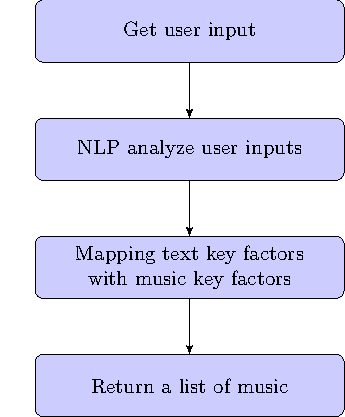
\includegraphics[width=4 in]{images/workflowg}
\caption{General Workflow}
\label{workflowg}
\end{figure}

\section{Thesis Outline}
\label{sec:outline}

In this project paper, five sections will be used to introduce and analyze the proposed music recommendation system.

\begin{itemize}
  \item The introduction will be mainly talking about the motivation of the project. Popular music services will also be introduced and analyzed. Besides motivation and popular music services, the expected goal of the music recommendation system and the general process steps will also be explained.
  \item The related work section will be mainly introducing similar studies. Each study will be introduced and analyzed toward their progress and limitations.
  \item The method section will be mainly about how is the system being build. Packages and tools used to build the system will also be introduced.
  \item The experiment section will be mainly talking about the evaluation of the system. The evaluation process and final results will be introduced and analyzed.
  \item Finally, the key findings and general ideas will be wrapped up in the conclusion section.
\end{itemize}
